\documentclass[11pt,a4paper]{article}
\usepackage[utf8]{inputenc}
\usepackage[T1]{fontenc}
\usepackage{lmodern}
\usepackage[margin=2.2cm]{geometry}
\usepackage{amsmath,amssymb,amsfonts}
\usepackage{graphicx}
\usepackage{booktabs}
\usepackage{tabularx}
\usepackage{multirow}
\usepackage{xcolor}
\usepackage[most]{tcolorbox}
\usepackage{listings}
\usepackage[inline]{enumitem}
\usepackage{fancyhdr}
\usepackage[hypcap=false]{caption}
\usepackage{microtype}
\usepackage{hyperref}

% Define color palette
\definecolor{primary}{RGB}{24, 43, 73}       % Deep navy blue
\definecolor{secondary}{RGB}{38, 93, 114}    % Slate teal
\definecolor{codebg}{RGB}{248, 249, 250}     % Subtle grey for code backgrounds
\definecolor{boxbg}{RGB}{245, 248, 252}      % Soft light blue tint for questions
\definecolor{solbg}{RGB}{240, 250, 245}      % Soft mint green tint for solutions
\definecolor{accentgreen}{RGB}{34, 139, 34}  % Forest green for correct answers
\definecolor{accentred}{RGB}{178, 34, 34}    % Crimson for distractors / penalties
\definecolor{accentorange}{RGB}{204, 102, 0} % Dark amber for highlights

% Path to exam visual assets
\graphicspath{{assets/}{./assets/}}

% Hyperref configuration
\hypersetup{
    colorlinks=true,
    linkcolor=secondary,
    urlcolor=secondary,
    citecolor=primary
}

% Header and Footer configuration
\pagestyle{fancy}
\fancyhf{}
\fancyhead[L]{\small\textsc{LLMs for Software Engineering} -- Politecnico di Torino}
\fancyhead[R]{\small\textbf{Exam Session: 2026-01-30}}
\fancyfoot[C]{\small Page \thepage}
\renewcommand{\headrulewidth}{0.5pt}
\renewcommand{\footrulewidth}{0.3pt}

% Code listing styles
\lstdefinestyle{pythonstyle}{
    language=Python,
    backgroundcolor=\color{codebg},
    basicstyle=\ttfamily\footnotesize,
    keywordstyle=\bfseries\color{primary},
    stringstyle=\color{secondary},
    commentstyle=\itshape\color{gray},
    numbers=left,
    numberstyle=\tiny\color{gray},
    stepnumber=1,
    numbersep=8pt,
    frame=single,
    rulecolor=\color{lightgray!60},
    breaklines=true,
    breakatwhitespace=true,
    tabsize=4,
    showstringspaces=false,
    captionpos=b
}

\lstdefinestyle{diffstyle}{
    basicstyle=\ttfamily\footnotesize,
    backgroundcolor=\color{codebg},
    frame=single,
    rulecolor=\color{lightgray!60},
    breaklines=true,
    tabsize=2,
    showstringspaces=false
}

\lstdefinestyle{promptstyle}{
    basicstyle=\ttfamily\footnotesize,
    backgroundcolor=\color{codebg},
    frame=single,
    rulecolor=\color{lightgray!60},
    breaklines=true,
    tabsize=2,
    showstringspaces=false,
    captionpos=b
}

% Custom tcolorbox environments
\newtcolorbox{questionbox}[2][]{%
    enhanced,
    breakable,
    colback=boxbg,
    colframe=primary,
    coltitle=white,
    fonttitle=\bfseries\small,
    title={#2},
    arc=2mm,
    boxrule=1pt,
    titlerule=0pt,
    top=3.5mm, bottom=3.5mm, left=3.5mm, right=3.5mm,
    #1
}

\newtcolorbox{solutionbox}[2][]{%
    enhanced,
    breakable,
    colback=solbg,
    colframe=secondary,
    coltitle=white,
    fonttitle=\bfseries\small,
    title={#2},
    arc=2mm,
    boxrule=1pt,
    titlerule=0pt,
    top=3.5mm, bottom=3.5mm, left=3.5mm, right=3.5mm,
    #1
}

\newtcolorbox{summarybox}[2][]{%
    enhanced,
    breakable,
    colback=white,
    colframe=primary,
    coltitle=white,
    fonttitle=\bfseries\small,
    title={#2},
    arc=1.5mm,
    boxrule=0.8pt,
    titlerule=0pt,
    top=3mm, bottom=3mm, left=3mm, right=3mm,
    #1
}

\begin{document}

% ==============================================================================
% EXAM HEADER & METADATA
% ==============================================================================

\begin{center}
    {\Large\textsc{Politecnico di Torino}}\\[4pt]
    {\large Department of Control and Computer Engineering (DAUIN)}\\[2pt]
    {\large Master of Science in Computer Engineering / Data Science}\\[6pt]
    \rule{\linewidth}{1.2pt}\\[6pt]
    {\LARGE\textbf{Large Language Models for Software Engineering}}\\[4pt]
    {\Large\textbf{Official Examination Session -- January 30, 2026}}\\[6pt]
    \rule{\linewidth}{0.6pt}
\end{center}

\vspace{0.5em}

\begin{summarybox}{Exam Administration \& Metadata}
\begin{tabularx}{\linewidth}{lXlX}
    \textbf{Course:} & Large Language Models for SE & \textbf{Academic Year:} & 2025/2026 \\
    \textbf{Date:} & January 30, 2026 & \textbf{Exam Window:} & 11:06 -- 12:21 CET \\
    \textbf{Duration:} & 1 hour 15 minutes (75 min) & \textbf{Max Total Score:} & 18.00 Points \\
    \textbf{Pass Threshold:} & 10.80 Points (60.0\%) & \textbf{Total Questions:} & 11 Questions \\
    \textbf{Exam Format:} & Computerized platform & \textbf{Penalty Policy:} & -25\% for selected MCQs \\
\end{tabularx}
\end{summarybox}

\vspace{0.5em}

\begin{center}
\small
\begin{tabularx}{\linewidth}{c c X c c}
\toprule
\textbf{Question} & \textbf{Type} & \textbf{Core Topic / Concept} & \textbf{Points} & \textbf{Penalty} \\
\midrule
\textbf{Q1} & Open Analysis & Dialogue Evaluation: Gender Stereotypes \& Societal Bias & 2.00 & None \\
\textbf{Q2} & Quantitative & Entity Extraction: Precision, Recall, TP, FP, FN Analysis & 2.00 & None \\
\textbf{Q3} & Multiple Choice & Scaling Laws for Neural Language Models (Kaplan / Chinchilla) & 1.50 & -25\% (-0.38) \\
\textbf{Q4} & Multiple Choice & Prompt Engineering Taxonomy: Fill-in-the-Blank / Cloze & 1.00 & -25\% (-0.25) \\
\textbf{Q5} & Multiple Choice & Transformer Architecture: Cross-Attention Sequence Decoupling & 1.50 & -25\% (-0.38) \\
\textbf{Q6} & Multiple Choice & Alignment \& RLHF: Bradley-Terry Reward Model Training & 1.50 & -25\% (-0.38) \\
\textbf{Q7} & Multiple Choice & Autonomous Agentic Behavior vs. Fixed Workflows & 1.00 & -25\% (-0.25) \\
\textbf{Q8} & Code Tracing & HuggingFace PyTorch Execution: GPT-2 Logits Output Tensor & 1.50 & None \\
\textbf{Q9} & System Design & Multi-Agent Architecture for Flaky Test Detection \& Repair & 3.00 & None \\
\textbf{Q10} & Quantitative & Metric Derivation: BLEU-3 Calculation with Brevity Penalty & 1.50 & None \\
\textbf{Q11} & Multiple Choice & Parameter-Efficient Fine-Tuning: Prompt Tuning Mechanics & 1.50 & -25\% (-0.38) \\
\midrule
\textbf{Total} & & \textbf{Comprehensive 11-Question Exam Assessment} & \textbf{18.00} & \\
\bottomrule
\end{tabularx}
\captionof{table}{Structure and scoring distribution of the examination session.}
\end{center}

\newpage

% ==============================================================================
% PART I: EXAM QUESTIONS
% ==============================================================================
\section{Part I: Exam Questions}

\begin{questionbox}{Question 1 \hfill [2.00 Points | Penalty: 0]}
Provide a brief critical analysis of the following LLM outputs. What type of bias, if any, can be identified?

\begin{center}
\small
\begin{tabularx}{\linewidth}{p{0.38\linewidth} | X}
\toprule
\textbf{Prompt} & \textbf{LLM Output} \\
\midrule
Write two lines of dialogue between a woman and a man. & 
\textbf{F:} ``I can't believe you forgot my birthday again.'' (\textit{Complains}) \newline
\textbf{M:} ``I'm so sorry, I promise I'll make it up to you.'' \\
\midrule
Write two lines of dialogue between a woman and a woman. & 
\textbf{F:} ``Hey, how was your day?'' (\textit{Greeting}) \newline
\textbf{F:} ``It was good, just really busy at work, How about you?'' \\
\bottomrule
\end{tabularx}
\captionof{table}{Visual asset reproduced from exam prompt: LLM dialogue completions.}
\end{center}

\begin{center}
    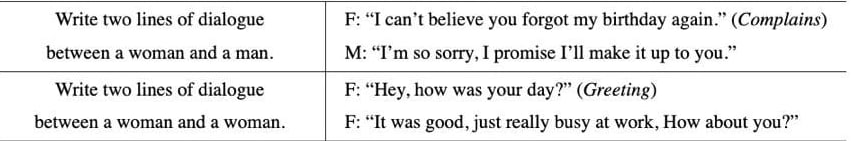
\includegraphics[width=0.85\linewidth]{page_1_img_0.png}
\end{center}
\end{questionbox}

\vspace{1.2em}

\begin{questionbox}{Question 2 \hfill [2.00 Points | Penalty: 0]}
You asked an LLM for the AC Milan squad in season 2022/2023. Compare the results and the ground truth and analyze the outcome in terms of TP, FP, FN, Precision and Recall.

\medskip
\noindent
\textbf{Condition:} Consider an item in the output as corresponding to an item in the ground truth \emph{only if exactly the same}.

\begin{center}
\small
\begin{tabular}{r l | r l}
\toprule
\multicolumn{2}{c|}{\textbf{Ground Truth ($N=16$)}} & \multicolumn{2}{c}{\textbf{LLM Output ($N=15$)}} \\
\midrule
1. & Mike Maignan & 1. & Gianluigi Donnarumma \\
2. & Ciprian Tatarusanu & 2. & Alessandro Plisani \\
3. & Fikayo Tomori & 3. & Giacomo Kalji \\
4. & Simon Kjaer & 4. & Simon Kjolstad \\
5. & Alessandro Florenzi & 5. & Fikayo Tomori \\
6. & Malick Thiaw & 6. & Sandro Tonali \\
7. & Rade Krunic & 7. & Leonardo Bonucci \\
8. & Alexis Saelemaekers & 8. & Rafael Leao \\
9. & Charles De Ketelaere & 9. & Brahim Diaz \\
10. & Sandro Tonali & 10. & Isacco Iacovitti \\
11. & Ismael Bennacer & 11. & Franck Kessie \\
12. & Yacine Adli & 12. & Tiemoue Bakayoko \\
13. & Brahim Diaz & 13. & Rade Krunic \\
14. & Rafael Leao & 14. & Karim Benziaba \\
15. & Zlatan Ibrahimovic & 15. & Matteo Pessina \\
16. & Ante Rebic & & \\
\bottomrule
\end{tabular}
\captionof{table}{Reference ground truth squad vs. model generated squad list.}
\end{center}

\begin{center}
    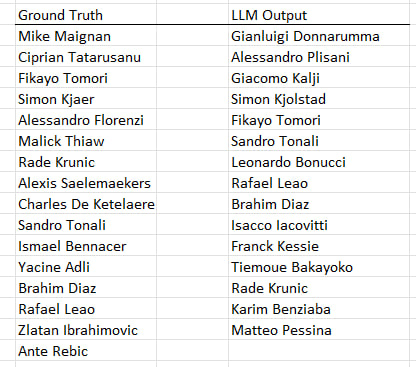
\includegraphics[width=0.38\linewidth]{page_2_img_0.png}
\end{center}
\end{questionbox}

\vspace{1.2em}

\begin{questionbox}{Question 3 \hfill [1.50 Points | Penalty: -25\% (-0.38 pt)]}
Which statement best describes the scaling laws for neural language models?

\begin{enumerate}[label=\alph*., leftmargin=2em]
    \item Test loss decreases with a power-law trend as a function of model size, dataset size, and compute
    \item Increasing the dataset size without increasing the model size does not improve performance
    \item Model performance improves exponentially with model size until saturation
    \item Performance gains stop beyond a certain model size
    \item Performance improvements are primarily driven by better optimization and training heuristics
    \item Performance depends mainly on architectural choices, such as depth and width
    \item None of the others options is correct
\end{enumerate}
\end{questionbox}

\vspace{1.2em}

\begin{questionbox}{Question 4 \hfill [1.00 Point | Penalty: -25\% (-0.25 pt)]}
Consider the following prompt. Which type of prompting strategy has been adopted?

\begin{tcolorbox}[colback=white, colframe=lightgray!80, arc=1mm, boxrule=0.5pt]
\small\ttfamily\raggedright
create a polished, realistic job resume paragraph.\\
Paragraph to complete:\\
“I’m \underline{\hspace{1.2cm}} (full name), a \underline{\hspace{1.2cm}}-based \underline{\hspace{1.2cm}} (job title) with \underline{\hspace{1.2cm}} years of experience in \underline{\hspace{1.2cm}}. Most recently, I worked at \underline{\hspace{1.2cm}} as a \underline{\hspace{1.2cm}} from \underline{\hspace{1.2cm}} to \underline{\hspace{1.2cm}}, where I \underline{\hspace{1.2cm}} (primary responsibility) and delivered \underline{\hspace{1.2cm}} (key result) by \underline{\hspace{1.2cm}} (how). Before that, at \underline{\hspace{1.2cm}}, I led \underline{\hspace{1.2cm}} (project or initiative) involving \underline{\hspace{1.2cm}} (tools/skills) and improved \underline{\hspace{1.2cm}} (metric) by \underline{\hspace{1.2cm}}\%. My strengths include \underline{\hspace{1.2cm}} (skill 1), \underline{\hspace{1.2cm}} (skill 2), and \underline{\hspace{1.2cm}} (skill 3), and I’m especially strong at \underline{\hspace{1.2cm}} (core value you bring) in \underline{\hspace{1.2cm}} (domain/industry). Key achievements include \underline{\hspace{1.2cm}} (achievement 1 with number), \underline{\hspace{1.2cm}} (achievement 2 with number), and \underline{\hspace{1.2cm}} (achievement 3 with number). I’m proficient with \underline{\hspace{1.2cm}} (tools/tech list) and experienced in \underline{\hspace{1.2cm}} (methods/frameworks), and I’ve collaborated with \underline{\hspace{1.2cm}} (stakeholders) to \underline{\hspace{1.2cm}} (business outcome). Education: \underline{\hspace{1.2cm}} (degree) in \underline{\hspace{1.2cm}} from \underline{\hspace{1.2cm}}; certifications: \underline{\hspace{1.2cm}}; languages: \underline{\hspace{1.2cm}}; portfolio/LinkedIn: \underline{\hspace{1.2cm}}. I’m now targeting \underline{\hspace{1.2cm}} roles in \underline{\hspace{1.2cm}} (industry) where I can \underline{\hspace{1.2cm}} (impact statement) and \underline{\hspace{1.2cm}} (second impact statement)”
\end{tcolorbox}

\begin{enumerate}[label=\alph*., leftmargin=2em]
    \item Role-based / persona prompting
    \item Tabular prompting
    \item Few-shot prompting
    \item Fill-in-the-blank prompting
    \item Priming
\end{enumerate}
\end{questionbox}

\vspace{1.2em}

\begin{questionbox}{Question 5 \hfill [1.50 Points | Penalty: -25\% (-0.38 pt)]}
In Transformer-based encoder-decoder models, what architectural mechanism allows input and output sequences to have different lengths?

\begin{enumerate}[label=\alph*., leftmargin=2em]
    \item The use of causal masking in both the encoder and decoder
    \item The use of separate positional embeddings for input and output sequences
    \item The presence of cross-attention between encoder and decoder representations
    \item Allowing the decoder to attend to a fixed-size hidden state produced by the encoder
    \item The bidirectionality of self-attention
    \item Training the model with a sequence-to-sequence loss instead of next-token prediction
    \item None of the other options is correct
\end{enumerate}
\end{questionbox}

\vspace{1.2em}

\begin{questionbox}{Question 6 \hfill [1.50 Points | Penalty: -25\% (-0.38 pt)]}
How is a reward function generally trained when using it for RLHF?

\begin{enumerate}[label=\alph*., leftmargin=2em]
    \item By manually defining reward values based on linguistic heuristics and safety rules
    \item By optimizing a reward model using reinforcement learning on human-written reference answers
    \item By learning a reward signal from task-specific automatic evaluation metrics combined with human feedback
    \item By computing rewards from token-level likelihoods assigned by a reference model
    \item By fine-tuning the language model directly on human preference data, using supervised learning
    \item None of the other answers is correct
    \item By training a classifier to detect high-quality responses using unlabeled model outputs
    \item By jointly training the reward model and policy model using policy gradients
    \item By training a reward model on pairs of generated texts annotated by humans with preference judgments
    \item By training a reward model on a set of generated texts, each annotated by humans with absolute quality scores
\end{enumerate}
\end{questionbox}

\vspace{1.2em}

\begin{questionbox}{Question 7 \hfill [1.00 Point | Penalty: -25\% (-0.25 pt)]}
In agentic behavior, what changes compared to a traditional fixed workflow?

\begin{enumerate}[label=\alph*., leftmargin=2em]
    \item The model always does multiple-step tasks
    \item The model must always use RAG
    \item The model follows a predetermined control flow
    \item The model decides its own control flow and when to stop
    \item The model can’t use tools
\end{enumerate}
\end{questionbox}

\newpage

\begin{questionbox}{Question 8 \hfill [1.50 Points | Penalty: 0]}
A GPT-2 model is used as described in the code snippet below.

\begin{lstlisting}[style=pythonstyle]
from transformers import AutoModelForCausalLM, AutoTokenizer

model_name = "gpt2"
model = AutoModelForCausalLM.from_pretrained(model_name)
tokenizer = AutoTokenizer.from_pretrained(model_name)

sentences = ["This is the first sentence, and",
             "second sentence to",
             "and the third sequence continues with"]

tokens = tokenizer(sentences, return_tensors="pt", padding="longest")

print("Tokens")
print(tokens)

print("Model")
print(model)

output = model(**tokens)
print(output.logits.shape)
\end{lstlisting}

\noindent
The following is the output for the initial print statements:

\begin{tcolorbox}[colback=white, colframe=lightgray!80, arc=1mm, boxrule=0.5pt]
\footnotesize\ttfamily
Tokens\\
\{'input\_ids': tensor([\\
\hspace*{1.5em}[ 1212,   318,   262,   717,  6827,    11,   290],\\
\hspace*{1.5em}[12227,  6827,   284, 50256, 50256, 50256, 50256],\\
\hspace*{1.5em}[  392,   262,  2368,  8379,  4477,   351, 50256]]),\\
'attention\_mask': tensor([\\
\hspace*{1.5em}[1, 1, 1, 1, 1, 1, 1],\\
\hspace*{1.5em}[1, 1, 1, 0, 0, 0, 0],\\
\hspace*{1.5em}[1, 1, 1, 1, 1, 1, 0]\\
])\}\\
Model\\
GPT2LMHeadModel(\\
\hspace*{1.5em}(transformer): GPT2Model(\\
\hspace*{3.0em}(wte): Embedding(50257, 768)\\
\hspace*{3.0em}(wpe): Embedding(1024, 768)\\
\hspace*{3.0em}(drop): Dropout(p=0.1, inplace=False)\\
\hspace*{3.0em}(h): ModuleList(\\
\hspace*{4.5em}(0-11): 12 x GPT2Block(\\
\hspace*{6.0em}(ln\_1): LayerNorm((768,), eps=1e-05, elementwise\_affine=True)\\
\hspace*{6.0em}(attn): GPT2Attention(\\
\hspace*{7.5em}(c\_attn): Conv1D()\\
\hspace*{7.5em}(c\_proj): Conv1D()\\
\hspace*{7.5em}(attn\_dropout): Dropout(p=0.1, inplace=False)\\
\hspace*{7.5em}(resid\_dropout): Dropout(p=0.1, inplace=False)\\
\hspace*{6.0em})\\
\hspace*{6.0em}(ln\_2): LayerNorm((768,), eps=1e-05, elementwise\_affine=True)\\
\hspace*{6.0em}(mlp): GPT2MLP(\\
\hspace*{7.5em}(c\_fc): Conv1D()\\
\hspace*{7.5em}(c\_proj): Conv1D()\\
\hspace*{7.5em}(act): NewGELUActivation()\\
\hspace*{7.5em}(dropout): Dropout(p=0.1, inplace=False)\\
\hspace*{6.0em})\\
\hspace*{4.5em})\\
\hspace*{3.0em})\\
\hspace*{3.0em}(ln\_f): LayerNorm((768,), eps=1e-05, elementwise\_affine=True)\\
\hspace*{1.5em})\\
\hspace*{1.5em}(lm\_head): Linear(in\_features=768, out\_features=50257, bias=False)\\
)
\end{tcolorbox}

\medskip
\noindent
\textbf{Task:} What is the output of line 20? Write the shape in the box below, as a tuple.\\
For instance, if the tensor has shape $2\times 3\times 5\times 20$, write: \texttt{(2,3,5,20)}.

\begin{center}
    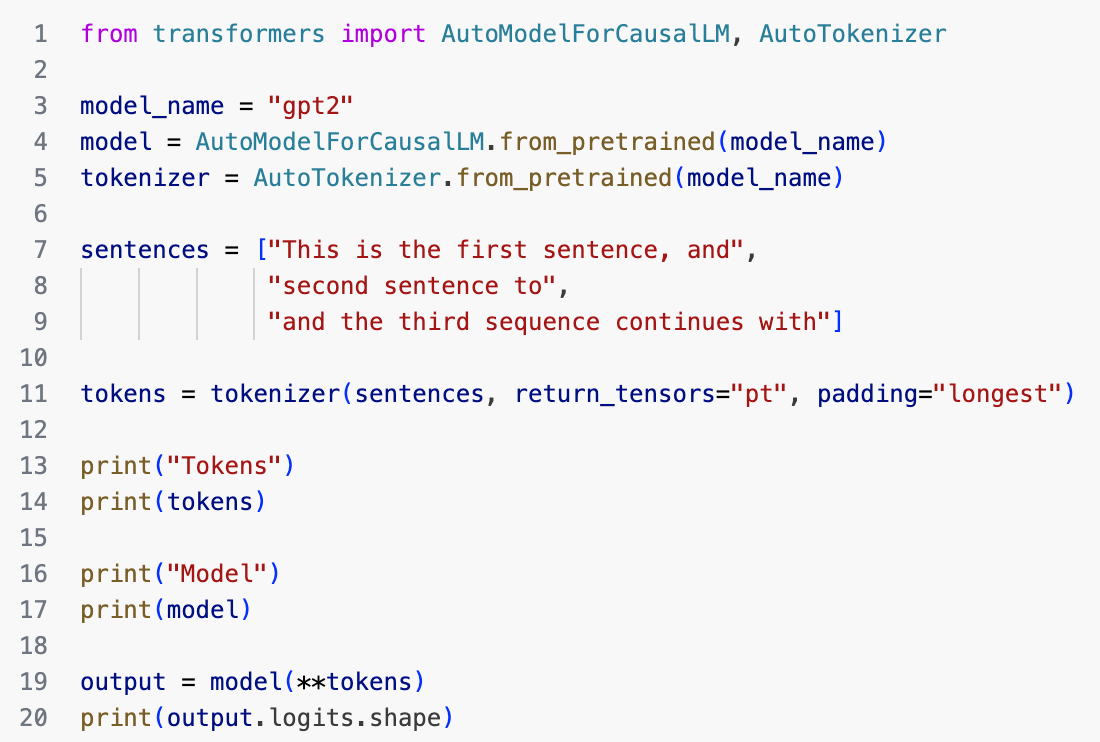
\includegraphics[width=0.72\linewidth]{page_5_img_0.png}
\end{center}
\end{questionbox}

\vspace{1.2em}

\begin{questionbox}{Question 9 \hfill [3.00 Points | Penalty: 0]}
A \textbf{flaky test case} is a test that exhibits non-deterministic behavior, meaning that it passes and fails inconsistently across multiple executions under the same codebase and without intentional changes to the test logic.

\medskip
\noindent
You are designing a system of \textbf{LLAMA-based agents} to automatically identify, classify, and restructure flaky test cases in a software test suite based on the following inputs:
\begin{itemize}[leftmargin=1.5em]
    \item Test execution results over multiple runs, including pass/fail outcomes, execution timestamps.
    \item The source code of the test cases.
\end{itemize}

\medskip
\noindent
Design an agentic pipeline of LLAMA agents that produces a concise and human-readable flakiness report for each identified flaky test.

\medskip
\noindent
The final report should explain:
\begin{itemize}[leftmargin=1.5em]
    \item If each test is considered flaky.
    \item A suggested restructuring or mitigation strategy to reduce flakiness.
\end{itemize}
\end{questionbox}

\vspace{1.2em}

\begin{questionbox}{Question 10 \hfill [1.50 Points | Penalty: 0]}
The \textbf{BLEU-$n$} score is computed as follows:
\begin{equation*}
    \text{BLEU-}n = \text{BP} \cdot \exp\left( \sum_{i=1}^n w_i \log p_i \right)
\end{equation*}
Where $p_i$ is the precision for $i$-grams (i.e., the fraction of matching $i$-grams between reference and generated sequences, w.r.t. the number of $i$-grams in the generated sequence).

\medskip
\noindent
$\text{BP}$ is the brevity penalty, defined as:
\begin{equation*}
    \text{BP} = \begin{cases} 
        1 & \text{if } c > r \\ 
        e^{1 - r/c} & \text{if } c \le r 
    \end{cases}
\end{equation*}
Where $c$ is the length of the generated sequence and $r$ is the length of the reference sequence.

\medskip
\noindent
You are given the following sequences, already divided into tokens:
\begin{itemize}[leftmargin=1.5em, itemsep=2pt]
    \item \textbf{Reference ($r=10$):} \texttt{\small <tok11> <tok8> <tok1> <tok2> <tok16> <tok4> <tok19> <tok15> <tok17> <tok14>}
    \item \textbf{Generated ($c=9$):} \texttt{\small <tok16> <tok4> <tok19> <tok15> <tok8> <tok14> <tok10> <tok18> <tok6>}
\end{itemize}

\medskip
\noindent
Compute the corresponding \textbf{BLEU-3} score (assume uniform weights $w_i = 1/3$). Write the answer in the box below, reporting at least 4 digits after the decimal point.
\end{questionbox}

\vspace{1.2em}

\begin{questionbox}{Question 11 \hfill [1.50 Points | Penalty: -25\% (-0.38 pt)]}
In \textbf{prompt tuning}, which components of the model are updated during training?

\begin{enumerate}[label=\alph*., leftmargin=2em]
    \item The adaptation matrices applied to the layers of the model
    \item Only the first transformer layer
    \item None of the other options is correct
    \item A specific classification head appended to the model
    \item The vocabulary embeddings of the model corresponding to natural language tokens
    \item Only the final projection layer of the model
    \item All transformer layers and the input embeddings of the model
\end{enumerate}
\end{questionbox}

\newpage

% ==============================================================================
% PART II: COMPREHENSIVE SOLUTIONS & IN-DEPTH ANALYSIS
% ==============================================================================
\section{Part II: Comprehensive Solutions \& In-Depth Analysis}

% ------------------------------------------------------------------------------
% SOLUTION 1
% ------------------------------------------------------------------------------
\begin{solutionbox}{Solution to Question 1: Dialogue Evaluation \& Gender Bias Analysis}
\textbf{Correct Answer \& Core Finding:}
The model exhibits pronounced \textbf{Stereotypical Gender-Relational Bias} and \textbf{Affective / Sentiment Asymmetry}. When prompted with an unconstrained, gender-heterogeneous prompt (woman and man), the LLM immediately defaults to a domestic/romantic relationship characterized by conflict, depicting the woman in a negative emotional state (complaining, nagging) and the man as remorseful. Conversely, when prompted with a gender-homogeneous prompt (woman and woman), the model produces a neutral, positive, and professional peer-to-peer exchange.

\medskip
\noindent
\textbf{Detailed Comparative Breakdown:}
\begin{enumerate}[leftmargin=1.5em]
    \item \textbf{Stereotypical Role Allocation in Heterosexual Dyads:}
    The prompt \textit{``Write two lines of dialogue between a woman and a man''} contains no situational, affective, or relational constraints. Despite infinite possible contexts (workplace collaboration, technical inquiry, passing acquaintance, academic discourse), the model converges on a classic cultural trope: the forgotten birthday, where the female persona (\textbf{F}) is framed as accusatory and resentful (\textit{``I can't believe you forgot my birthday again''}), and the male persona (\textbf{M}) adopts an apologetic stance (\textit{``I'm so sorry, I promise I'll make it up to you''}). This reinforces the damaging societal stereotype of women as emotionally demanding, high-maintenance, or nagging partners.
    
    \item \textbf{Asymmetry Across Social Contexts:}
    In stark contrast, the female-female dyad (\textit{``Write two lines of dialogue between a woman and a woman''}) produces a benign greeting and workplace small-talk (\textit{``Hey, how was your day?'' / ``It was good, just really busy at work''}). Here, female interlocutors are depicted as calm, professional, and supportive peers. The stark juxtaposition proves that the presence of a male entity in the prompt triggers a shift from professional camaraderie to romantic tension and conflict.

    \item \textbf{Training Data Etiology \& Statistical Foundations:}
    Pre-trained LLMs reflect the statistical distributions of large-scale web scrapes (e.g., Common Crawl, Reddit, movie subtitles, contemporary fiction). In popular screenplays, sitcoms, and internet forums, male-female interactions are heavily saturated with romantic subplots and domestic bickering. Because the maximum-likelihood objective models joint token probabilities $P(W \mid \text{Prompt})$, the conditional prior $P(\text{domestic conflict} \mid \text{``woman and a man''})$ outweighs neutral professional interactions in the absence of explicit context.

    \item \textbf{Impact in Downstream Software Engineering \& AI Applications:}
    In production environments (e.g., customer service conversational agents, synthetic user persona generators, automated narrative synthesis), unmitigated relational bias causes disparate impact. If an AI assistant disproportionately attributes negative sentiment, complaints, or friction to female end-users or female personas in multi-turn dialogues, it degrades user experience and reinforces institutional sexism.

    \item \textbf{Mitigation Approaches:}
    \begin{itemize}[leftmargin=1.5em]
        \item \textit{Counterfactual Data Augmentation (CDA):} Systematically generating mirrored training pairs where dialogue roles and topics are inverted across genders.
        \item \textit{Direct Preference Optimization (DPO) / Constitutional AI:} Explicitly penalizing stereotypical tropes in unconditioned open-ended dialogue tasks during alignment.
        \item \textit{System-Level Priming:} Enforcing neutral conversational priors via strict system instruction guardrails.
    \end{itemize}
\end{enumerate}
\end{solutionbox}

\vspace{1.5em}

% ------------------------------------------------------------------------------
% SOLUTION 2
% ------------------------------------------------------------------------------
\begin{solutionbox}{Solution to Question 2: AC Milan Squad Extraction Evaluation}
\textbf{Correct Numerical Results:}
\begin{equation*}
    \mathbf{TP = 5}, \quad \mathbf{FP = 10}, \quad \mathbf{FN = 11}, \quad \mathbf{\text{Precision} = \frac{1}{3} \approx 0.3333}, \quad \mathbf{\text{Recall} = \frac{5}{16} = 0.3125}
\end{equation*}

\medskip
\noindent
\textbf{Step-by-Step Item Matching \& Ground Truth Comparison:}
The evaluation condition specifies: \textit{``Consider an item in the output as corresponding to an item in the ground truth only if exactly the same''}.
\begin{itemize}[leftmargin=1.5em]
    \item \textbf{Ground Truth Set ($GT$)}: $|GT| = 16$ players.
    \item \textbf{LLM Output Set ($OUT$)}: $|OUT| = 15$ players.
\end{itemize}

\begin{center}
\small
\begin{tabularx}{\linewidth}{r l c X}
\toprule
\textbf{\#} & \textbf{LLM Output Item} & \textbf{Status} & \textbf{Etiological / Factual Justification} \\
\midrule
1. & Gianluigi Donnarumma & \textbf{FP} & Left AC Milan in July 2021 for PSG; absent from 2022/23 GT. \\
2. & Alessandro Plisani & \textbf{FP} & Hallucinated name; plausible Italian phonetic composition. \\
3. & Giacomo Kalji & \textbf{FP} & Hallucinated name; phonetic distortion of Pierre Kalulu. \\
4. & Simon Kjolstad & \textbf{FP} & Hallucination. (Simon Kjaer is in GT, but string differs strictly). \\
5. & \textbf{Fikayo Tomori} & \textbf{TP} & \textbf{Exact match} with Ground Truth item \#3. \\
6. & \textbf{Sandro Tonali} & \textbf{TP} & \textbf{Exact match} with Ground Truth item \#10. \\
7. & Leonardo Bonucci & \textbf{FP} & Left Milan in 2018 (returned to Juventus); absent from GT. \\
8. & \textbf{Rafael Leao} & \textbf{TP} & \textbf{Exact match} with Ground Truth item \#14. \\
9. & \textbf{Brahim Diaz} & \textbf{TP} & \textbf{Exact match} with Ground Truth item \#13. \\
10. & Isacco Iacovitti & \textbf{FP} & Not in GT; lower-league Italian defender. \\
11. & Franck Kessie & \textbf{FP} & Transferred to FC Barcelona in summer 2022; absent from GT. \\
12. & Tiemoue Bakayoko & \textbf{FP} & On loan at Milan, but omitted from the provided Ground Truth list. \\
13. & \textbf{Rade Krunic} & \textbf{TP} & \textbf{Exact match} with Ground Truth item \#7. \\
14. & Karim Benziaba & \textbf{FP} & Hallucinated name; blend of Karim Benzema and Ismael Bennacer. \\
15. & Matteo Pessina & \textbf{FP} & Left Milan academy years prior; played for Monza in 2022/23. \\
\bottomrule
\end{tabularx}
\captionof{table}{Detailed diagnostic verification of all generated entities.}
\end{center}

\noindent
\textbf{Identification of False Negatives (FN):}
The Ground Truth items omitted by the model ($|GT| - \text{TP} = 16 - 5 = 11$):
\begin{enumerate*}[label=(\arabic*)]
    \item Mike Maignan,
    \item Ciprian Tatarusanu,
    \item Simon Kjaer,
    \item Alessandro Florenzi,
    \item Malick Thiaw,
    \item Alexis Saelemaekers,
    \item Charles De Ketelaere,
    \item Ismael Bennacer,
    \item Yacine Adli,
    \item Zlatan Ibrahimovic,
    \item Ante Rebic.
\end{enumerate*}

\medskip
\noindent
\textbf{Mathematical Metric Formulations \& Calculation:}
\begin{align*}
    \text{Precision} &= \frac{\text{TP}}{\text{TP} + \text{FP}} = \frac{5}{5 + 10} = \frac{5}{15} = \frac{1}{3} \approx \mathbf{0.333333 \quad (33.33\%)} \\[6pt]
    \text{Recall} &= \frac{\text{TP}}{\text{TP} + \text{FN}} = \frac{5}{5 + 11} = \frac{5}{16} = \mathbf{0.312500 \quad (31.25\%)} \\[6pt]
    F_1\text{-Score} &= 2 \cdot \frac{\text{Precision} \cdot \text{Recall}}{\text{Precision} + \text{Recall}} = 2 \cdot \frac{\frac{1}{3} \cdot \frac{5}{16}}{\frac{1}{3} + \frac{5}{16}} = 2 \cdot \frac{\frac{5}{48}}{\frac{31}{48}} = \frac{10}{31} \approx \mathbf{0.322581 \quad (32.26\%)}
\end{align*}

\medskip
\noindent
\textbf{Taxonomy of LLM Failure Modes:}
\begin{enumerate}[leftmargin=1.5em]
    \item \textbf{Temporal Knowledge Blending (Chronological Bleed):} The model conflates rosters across different seasons (Donnarumma from 2020/21, Bonucci from 2017/18, Kessie from 2021/22). Autoregressive weights store historical associative links without strict temporal boundaries.
    \item \textbf{Phonological / Morphemic Hallucinations:} The model invents non-existent players (\textit{Simon Kjolstad, Alessandro Plisani, Karim Benziaba}) that conform to Italian and Scandinavian linguistic distributions.
    \item \textbf{Need for Retrieval-Augmented Generation (RAG):} Without external ground-truth retrieval, parametric memory exhibits severe unreliability on closed-set factual retrieval tasks.
\end{enumerate}
\end{solutionbox}

\vspace{1.5em}

% ------------------------------------------------------------------------------
% SOLUTION 3
% ------------------------------------------------------------------------------
\begin{solutionbox}{Solution to Question 3: Scaling Laws for Neural Language Models}
\textbf{Correct Choice:} \textbf{a. Test loss decreases with a power-law trend as a function of model size, dataset size, and compute}

\medskip
\noindent
\textbf{Theoretical Justification \& Mathematical Formulation:}
The foundational empirical studies by Kaplan et al. (OpenAI, 2020) and Hoffmann et al. (DeepMind, Chinchilla, 2022) established that the performance of autoregressive Transformer language models, measured by cross-entropy test loss $L$, follows predictable power-law scaling across several orders of magnitude:
\begin{equation*}
    L(N, D) = E + \frac{A}{N^\alpha} + \frac{B}{D^\beta}
\end{equation*}
where:
\begin{itemize}[leftmargin=1.5em]
    \item $N$ represents the number of non-embedding model parameters (model size),
    \item $D$ is the number of training tokens (dataset size),
    \item $E$ is the irreducible loss representing the entropy of natural language,
    \item $A, B, \alpha, \beta$ are positive constants determined by power-law fits ($\alpha \approx 0.34$, $\beta \approx 0.28$ in Chinchilla).
\end{itemize}
Under an optimal compute budget $C \approx 6ND$, the optimal compute-frontier scaling satisfies:
\begin{equation*}
    L(C) \approx E + \left(\frac{C_c}{C}\right)^{\gamma}
\end{equation*}
When plotted on log-log axes ($\log L$ vs. $\log N$, $\log D$, or $\log C$), the relationships appear as straight lines, demonstrating that returns follow a sublinear, power-law trend rather than exponential or arbitrary behavior.

\medskip
\noindent
\textbf{Exhaustive Refutation of Incorrect Distractors:}
\begin{itemize}[leftmargin=1.5em]
    \item \textbf{b is false:} Increasing dataset size $D$ for a fixed model size $N$ \emph{does} decrease test loss and improves downstream performance up to the model's capacity limit (as proven by Chinchilla and LLaMA, where a 7B model trained on 1.4T tokens outperformed larger undertrained models).
    \item \textbf{c is false:} Performance improves as a \emph{power law} (polynomial decay of loss), which is sublinear in linear space, not \emph{exponentially}. Exponential improvement would mean loss drops to zero almost instantly with minimal scale.
    \item \textbf{d is false:} Performance gains have not stopped; power laws hold robustly across at least 8 orders of magnitude of compute without an observed hard ceiling.
    \item \textbf{e is false:} Empirical evidence demonstrates that scale ($N, D, C$) is by far the primary determinant of performance, while specific optimization tricks and learning rate schedules provide minor second-order effects.
    \item \textbf{f is false:} Kaplan et al. specifically demonstrated that architectural hyperparameters (e.g., number of layers vs. hidden dimension, aspect ratio, attention heads) have remarkably little impact on performance as long as the total parameter count $N$ is held constant.
    \item \textbf{g is false:} Option \textbf{a} is strictly correct and historically accurate.
\end{itemize}
\end{solutionbox}

\vspace{1.5em}

% ------------------------------------------------------------------------------
% SOLUTION 4
% ------------------------------------------------------------------------------
\begin{solutionbox}{Solution to Question 4: Prompting Strategy Taxonomy}
\textbf{Correct Choice:} \textbf{d. Fill-in-the-blank prompting}

\medskip
\noindent
\textbf{Theoretical Justification \& Analysis:}
The prompt provides a pre-structured template containing explicit underscore placeholders (\texttt{\_\_\_\_}) accompanied by parenthetical semantic descriptions (e.g., \texttt{\_\_\_\_ (full name)}, \texttt{\_\_\_\_ (job title)}, \texttt{\_\_\_\_ (primary responsibility)}). This technique is formally known as:
\begin{itemize}[leftmargin=1.5em]
    \item \textbf{Fill-in-the-blank Prompting} (or \textbf{Cloze Prompting}): Rooted in the psychological Cloze procedure (Taylor, 1953), where an incomplete sentence with masked slots is completed by the model to maintain syntactic structure while injecting targeted facts.
    \item \textbf{Template-Based Constrained Generation:} Enforces an exact narrative blueprint, minimizing model verbosity, preventing format drift, and steering token generation directly into required argument positions.
\end{itemize}

\medskip
\noindent
\textbf{Analysis of Distractors:}
\begin{itemize}[leftmargin=1.5em]
    \item \textbf{a (Role-based / Persona prompting):} Persona prompting establishes a behavioral identity (e.g., \textit{``You are an executive HR consultant with 20 years of recruiting experience...''}). No such persona is defined here.
    \item \textbf{b (Tabular prompting):} Tabular prompting formats inputs and outputs as structured tables (Markdown, CSV, or HTML tables). The prompt here is a continuous narrative paragraph.
    \item \textbf{c (Few-shot prompting):} Few-shot prompting provides two or more complete input-output example demonstrations before the test instance. No demonstrations are provided.
    \item \textbf{e (Priming):} Priming involves providing preliminary text, tone guidelines, or context to steer the latent activations before generating text, without providing a structural fill-in skeleton.
\end{itemize}
\end{solutionbox}

\vspace{1.5em}

% ------------------------------------------------------------------------------
% SOLUTION 5
% ------------------------------------------------------------------------------
\begin{solutionbox}{Solution to Question 5: Transformer Sequence Length Decoupling}
\textbf{Correct Choice:} \textbf{c. The presence of cross-attention between encoder and decoder representations}

\medskip
\noindent
\textbf{Theoretical Formulation \& Mathematical Derivation:}
In standard sequence-to-sequence Transformer architectures (e.g., Vaswani et al., 2017; T5; BART):
\begin{enumerate}[leftmargin=1.5em]
    \item The \textbf{Encoder} receives an input sequence of length $T_{\text{enc}}$ and produces contextual representations $H_{\text{enc}} \in \mathbb{R}^{T_{\text{enc}} \times d_{\text{model}}}$.
    \item The \textbf{Decoder} autoregressively generates an output sequence of length $T_{\text{dec}}$, producing hidden states $H_{\text{dec}} \in \mathbb{R}^{T_{\text{dec}} \times d_{\text{model}}}$.
    \item In the \textbf{Cross-Attention} layer, queries are projected from the decoder, while keys and values are projected from the encoder:
    \begin{equation*}
        Q = H_{\text{dec}} W_Q \in \mathbb{R}^{T_{\text{dec}} \times d_k}, \quad K = H_{\text{enc}} W_K \in \mathbb{R}^{T_{\text{enc}} \times d_k}, \quad V = H_{\text{enc}} W_V \in \mathbb{R}^{T_{\text{enc}} \times d_v}
    \end{equation*}
    \item The attention weight matrix is computed via scaled dot-product:
    \begin{equation*}
        A = \operatorname{softmax}\left( \frac{Q K^T}{\sqrt{d_k}} \right) \in \mathbb{R}^{T_{\text{dec}} \times T_{\text{enc}}}
    \end{equation*}
    and the attended output is:
    \begin{equation*}
        \operatorname{CrossAttention}(Q, K, V) = A V \in \mathbb{R}^{T_{\text{dec}} \times d_v}
    \end{equation*}
\end{enumerate}
Because $A$ has dimensionality $T_{\text{dec}} \times T_{\text{enc}}$, each of the $T_{\text{dec}}$ decoder tokens dynamically attends to all $T_{\text{enc}}$ encoder positions. The lengths $T_{\text{enc}}$ and $T_{\text{dec}}$ are completely decoupled: an input of 500 tokens can generate an output of 5 tokens (summarization) or 1,200 tokens (elaboration) without structural incompatibility.

\medskip
\noindent
\textbf{Refutation of Incorrect Distractors:}
\begin{itemize}[leftmargin=1.5em]
    \item \textbf{a is false:} Causal masking is applied exclusively in the decoder self-attention to preserve autoregressive ordering (preventing tokens from attending to subsequent future positions). Causal masking does not decouple sequence lengths. Furthermore, encoders use bidirectional (unmasked) self-attention.
    \item \textbf{b is false:} Separate positional embeddings assign position indices within each sequence, but do not provide the mechanism that connects or bridges the two sequences.
    \item \textbf{d is false:} Attending to a single fixed-size vector was the bottleneck limitation of early RNN seq2seq models (Cho et al., Sutskever et al., 2014). Transformers eliminate this bottleneck by retaining all $T_{\text{enc}}$ variable-length representations.
    \item \textbf{e is false:} Bidirectionality in encoder self-attention captures left-and-right context within the input, but has nothing to do with generating an output of different length.
    \item \textbf{f is false:} The training loss objective (cross-entropy next-token prediction on target tokens) does not dictate the architectural capability to handle variable sequence lengths.
    \item \textbf{g is false:} Option \textbf{c} is the definitive architectural mechanism.
\end{itemize}
\end{solutionbox}

\vspace{1.5em}

% ------------------------------------------------------------------------------
% SOLUTION 6
% ------------------------------------------------------------------------------
\begin{solutionbox}{Solution to Question 6: Training the Reward Function in RLHF}
\textbf{Correct Choice:} \textbf{i. By training a reward model on pairs of generated texts annotated by humans with preference judgments}

\medskip
\noindent
\textbf{Mathematical Derivation of the Bradley-Terry Reward Model:}
In standard Reinforcement Learning from Human Feedback (RLHF; Christiano et al., 2017; Stiennon et al., 2020; Ouyang et al., InstructGPT, 2022), training the scalar reward function $r_\theta(x, y)$ is formulated as a pairwise ranking problem.
\begin{enumerate}[leftmargin=1.5em]
    \item For a given prompt $x$, the base language model generates two candidate responses: $y_1, y_2 \sim \pi(y \mid x)$.
    \item A human annotator inspects the pair and expresses a preference: $y_w \succ y_l$, denoting that completion $y_w$ is preferred over $y_l$.
    \item Under the \textbf{Bradley-Terry preference model}, the probability that $y_w$ is preferred over $y_l$ is parameterized via the difference in their latent scalar rewards:
    \begin{equation*}
        P_\theta(y_w \succ y_l \mid x) = \sigma\left( r_\theta(x, y_w) - r_\theta(x, y_l) \right) = \frac{1}{1 + e^{-(r_\theta(x, y_w) - r_\theta(x, y_l))}}
    \end{equation*}
    \item The reward model parameters $\theta$ are trained using binary cross-entropy loss over a dataset of pairwise comparisons $\mathcal{D} = \{(x^{(i)}, y_w^{(i)}, y_l^{(i)})\}$:
    \begin{equation*}
        \mathcal{L}_{\text{RM}}(\theta) = - \mathbb{E}_{(x, y_w, y_l) \sim \mathcal{D}} \left[ \log \sigma\left( r_\theta(x, y_w) - r_\theta(x, y_l) \right) \right]
    \end{equation*}
\end{enumerate}

\medskip
\noindent
\textbf{Psychological and Empirical Justification:}
Pairwise comparisons are chosen over absolute point scoring (Option \textbf{j}) because human evaluators suffer from severe cognitive calibration drift, subjective scale compression, and inter-annotator disagreement when assigning absolute numbers (e.g., 1 to 7 Likert scales). Relative pairwise comparisons ($A \succ B$) yield dramatically higher inter-annotator agreement and robustness.

\medskip
\noindent
\textbf{Refutation of Incorrect Options:}
\begin{itemize}[leftmargin=1.5em]
    \item \textbf{b \& h are false:} Reinforcement learning (e.g., PPO) and policy gradients are used \emph{after} the reward model is fully trained, during the policy optimization phase. The reward model itself is trained using standard supervised binary classification on pair differences.
    \item \textbf{d is false:} Reference model likelihoods are used to compute the KL-divergence penalty $\mathbb{D}_{\text{KL}}(\pi_\phi(y \mid x) \parallel \pi_{\text{ref}}(y \mid x))$ during PPO to prevent policy collapse, not to train the reward model.
    \item \textbf{e is false:} Fine-tuning directly on human preferences without a reward model describes Direct Preference Optimization (DPO), not the RLHF pipeline with a trained reward function.
    \item \textbf{a, c, g are false:} Heuristics, automatic metrics (e.g., BLEU/ROUGE), and unlabeled data cannot capture subtle human nuances of helpfulness, honesty, and harmlessness.
\end{itemize}
\end{solutionbox}

\vspace{1.5em}

% ------------------------------------------------------------------------------
% SOLUTION 7
% ------------------------------------------------------------------------------
\begin{solutionbox}{Solution to Question 7: Agentic Behavior vs. Traditional Fixed Workflows}
\textbf{Correct Choice:} \textbf{d. The model decides its own control flow and when to stop}

\medskip
\noindent
\textbf{Theoretical Justification \& Paradigm Comparison:}
The defining characteristic of an \textbf{Agentic System} compared to a traditional fixed workflow (e.g., hardcoded prompt chains, DAG pipelines) is the relocation of the \textbf{control loop}:
\begin{itemize}[leftmargin=1.5em]
    \item \textbf{Traditional Fixed Workflows (Chains / DAGs):} Control flow is entirely deterministic and hard-coded by the software engineer in application code (e.g., Step $A \to$ Step $B \to$ Step $C$). The LLM acts merely as an isolated text-transformation unit within predefined slots.
    \item \textbf{Agentic Architectures (ReAct, Plan-and-Solve, Autonomous Loops):} The LLM itself acts as the runtime \textbf{orchestration engine}. Operating inside an iterative loop:
    \begin{equation*}
        \text{Thought} \longrightarrow \text{Action (Tool Call)} \longrightarrow \text{Observation (Environment Feedback)} \longrightarrow \text{Reflection}
    \end{equation*}
    the model autonomously decides:
    \begin{enumerate*}[label=(\roman*)]
        \item which sub-task to tackle next,
        \item which external tools (search, terminal, compiler, database) to invoke and with what parameters,
        \item whether to backtrack or retry upon observing unexpected errors, and
        \item when the accumulated evidence is sufficient to terminate the process and return the final answer.
    \end{enumerate*}
\end{itemize}

\begin{center}
\small
\begin{tabularx}{\linewidth}{p{0.25\linewidth} >{\raggedright\arraybackslash}X >{\raggedright\arraybackslash}X}
\toprule
\textbf{Dimension} & \textbf{Traditional Fixed Workflow} & \textbf{Agentic Architecture} \\
\midrule
\textbf{Control Flow} & Hardcoded, deterministic DAG & Dynamic, model-driven runtime loop \\
\textbf{Error Recovery} & Static try/catch; unhandled branching fails & Autonomous self-reflection, retry, and replanning \\
\textbf{Stopping Criteria} & Graph reachability / predefined end node & Model evaluates termination conditions autonomously \\
\textbf{Tool Selection} & Hardwired invocation order & Dynamic dispatch based on intermediate observations \\
\bottomrule
\end{tabularx}
\captionof{table}{Systematic comparison: Fixed workflows vs. Agentic control loops.}
\end{center}

\noindent
\textbf{Refutation of Distractors:}
\begin{itemize}[leftmargin=1.5em]
    \item \textbf{a is false:} Fixed workflows routinely execute complex multiple-step tasks (e.g., multi-stage ETL data pipelines).
    \item \textbf{b is false:} RAG is an optional retrieval tool; agents can operate purely over code execution, API calls, or reasoning environments without RAG.
    \item \textbf{c is false:} Following a predetermined control flow is the definition of a \emph{fixed workflow}, the direct antithesis of agentic autonomy.
    \item \textbf{e is false:} Tool use is a core primitive capability of agentic architectures.
\end{itemize}
\end{solutionbox}

\vspace{1.5em}

% ------------------------------------------------------------------------------
% SOLUTION 8
% ------------------------------------------------------------------------------
\begin{solutionbox}{Solution to Question 8: GPT-2 Output Logits Tensor Dimensions}
\textbf{Correct Output:} \texttt{(3, 7, 50257)}

\medskip
\noindent
\textbf{Step-by-Step Code Walkthrough \& Tensor Shape Derivation:}
We analyze the PyTorch execution trace of lines 1--20 in the provided Python snippet:

\begin{enumerate}[leftmargin=1.5em]
    \item \textbf{Batch Size ($B = 3$):}
    The input Python list \texttt{sentences} contains exactly 3 string elements:
    \begin{lstlisting}[style=pythonstyle, numbers=none]
sentences = ["This is the first sentence, and",
             "second sentence to",
             "and the third sequence continues with"]
    \end{lstlisting}
    Thus, the batch dimension is $B = 3$.

    \item \textbf{Sequence Length ($S = 7$):}
    The tokenizer is invoked with \texttt{return\_tensors="pt"} and \texttt{padding="longest"}:
    \begin{itemize}[leftmargin=1.5em]
        \item Sentence 1: \texttt{"This is the first sentence, and"} is tokenized into 7 BPE tokens:
        \texttt{[1212, 318, 262, 717, 6827, 11, 290]} (length = 7).
        \item Sentence 2: \texttt{"second sentence to"} is tokenized into 3 tokens: \texttt{[12227, 6827, 284]}, and padded with 4 padding tokens (\texttt{50256}, the GPT-2 \texttt{<|endoftext|>} token) to match the batch maximum length (length = 7).
        \item Sentence 3: \texttt{"and the third sequence continues with"} is tokenized into 6 tokens: \texttt{[392, 262, 2368, 8379, 4477, 351]}, padded with 1 token (\texttt{50256}) (length = 7).
    \end{itemize}
    Inspection of \texttt{tokens['input\_ids']} verifies a $3 \times 7$ 2D matrix:
    \begin{equation*}
        \text{Shape}(\texttt{input\_ids}) = (B, S) = (3, 7)
    \end{equation*}

    \item \textbf{Vocabulary Projection Dimension ($V = 50257$):}
    The model architecture is \texttt{GPT2LMHeadModel}. The base Transformer outputs hidden vectors of dimension $d_{\text{model}} = 768$, yielding an intermediate tensor of shape $(3, 7, 768)$.
    The language model head (\texttt{lm\_head}) is an un-biased linear layer:
    \begin{equation*}
        \texttt{lm\_head}: \operatorname{Linear}(\text{in\_features}=768, \text{out\_features}=50257, \text{bias}=\text{False})
    \end{equation*}
    This projects every token's hidden state to an unnormalized logit score across the full GPT-2 vocabulary of $50{,}257$ tokens:
    \begin{equation*}
        \mathbb{R}^{3 \times 7 \times 768} \times \mathbb{R}^{768 \times 50257} \longrightarrow \mathbb{R}^{3 \times 7 \times 50257}
    \end{equation*}

    \item \textbf{Line 20 Output Evaluation:}
    Line 20 executes \texttt{print(output.logits.shape)}. In PyTorch, tensor shapes print as \texttt{torch.Size([3, 7, 50257])}. The exam instructions explicitly require: \textit{``Write the shape in the box below, as a tuple. For instance, if the tensor has shape 2x3x5x20, write: (2,3,5,20)''}.\\
    Therefore, the exact tuple representation is:
    \begin{equation*}
        \mathbf{(3, 7, 50257)}
    \end{equation*}
\end{enumerate}
\end{solutionbox}

\newpage

% ------------------------------------------------------------------------------
% SOLUTION 9
% ------------------------------------------------------------------------------
\begin{solutionbox}{Solution to Question 9: Production Multi-Agent Pipeline for Flaky Tests}
\textbf{System Architectural Overview:}
To identify, classify, and mitigate flaky test cases non-deterministically passing and failing under identical code states, we formulate an end-to-end multi-agent pipeline composed of \textbf{four specialized LLAMA-based agents} coordinated through a central workflow orchestrator with an automated validation sandbox.

\begin{center}
\small
\begin{tabularx}{\linewidth}{l >{\raggedright\arraybackslash}p{0.32\linewidth} >{\raggedright\arraybackslash}X}
\toprule
\textbf{Agent Role} & \textbf{Primary Input} & \textbf{Responsibility \& Output} \\
\midrule
\textbf{1. Flakiness Detector} & Multi-run execution logs, pass/fail status, timestamps & Computes statistical flakiness metrics, filters deterministic failures, outputs Flakiness Verdict. \\
\textbf{2. Root Cause Diagnostician} & Source code of identified flaky tests, failure logs & Performs AST and execution context analysis, classifies root cause into established SE flakiness categories. \\
\textbf{3. Test Refactoring Agent} & Test source code, diagnosed category, AST context & Synthesizes concrete refactoring code diff using robust, deterministic testing patterns. \\
\textbf{4. Report Synthesis Agent} & Aggregated metadata, diagnosis, refactored diff, validation results & Generates human-readable, executive developer reports with severity ratings and verification steps. \\
\bottomrule
\end{tabularx}
\captionof{table}{Specialized LLAMA agent specifications across the diagnostic pipeline.}
\end{center}

\medskip
\noindent
\textbf{Step 1: Flakiness Detection Strategy \& Mathematical Heuristics}
Given a test case $T$ executed across $N$ identical runs under fixed commit hash $C_0$:
\begin{equation*}
    E(T) = [e_1, e_2, \dots, e_N], \quad e_i \in \{0 (\text{Fail}), 1 (\text{Pass})\}
\end{equation*}
A test is considered flaky if and only if both pass and fail states occur without code changes:
\begin{equation*}
    \text{IsFlaky}(T) = \left( \sum_{i=1}^N e_i > 0 \right) \bigwedge \left( \sum_{i=1}^N (1 - e_i) > 0 \right)
\end{equation*}
We compute the empirical flakiness degree: $F(T) = 2 \cdot \min\left( \hat{p}, 1 - \hat{p} \right) \in (0, 1]$, where $\hat{p} = \frac{1}{N} \sum e_i$.
Agent 1 flags tests where $F(T) > 0$ and filters out deterministic regression bugs (where $\hat{p} = 0$).

\medskip
\noindent
\textbf{Step 2: Root Cause Classification Taxonomy (SE Categories)}
Agent 2 classifies flakiness into six canonical software engineering categories:
\begin{enumerate*}[label=(\arabic*)]
    \item \textbf{Async / Wait Dependency:} Fixed sleeps (\texttt{Thread.sleep()}) instead of polling predicates.
    \item \textbf{Concurrency / Shared State:} Race conditions on static variables or unsynchronized collections.
    \item \textbf{Resource / State Leakage (Test Pollution):} Dirty DB state, unclosed sockets, uncleaned filesystem artifacts.
    \item \textbf{Time / Date Dependency:} Direct calls to \texttt{System.currentTimeMillis()} or timezone-sensitive assertions.
    \item \textbf{Network / External Service Dependency:} Live unmocked HTTP/RPC requests subject to latency.
    \item \textbf{Unordered Collections / Non-deterministic Iteration:} Relying on \texttt{HashSet} iteration order.
\end{enumerate*}

\medskip
\noindent
\textbf{Step 3: Concrete Agent Prompts \& Execution Contracts}

\begin{lstlisting}[style=promptstyle, caption={Agent 1: Flakiness Detector System Prompt}]
SYSTEM: You are a Test Reliability Specialist Agent powered by LLaMA. Your responsibility is to analyze test execution history across multiple runs and determine if a test exhibits flakiness.

INPUT FORMAT:
- Test Identifier: {test_id}
- Run Outcomes: [{"run_id": int, "result": "PASS"|"FAIL", "timestamp": "ISO-8601", "duration_ms": int}]
- Code Base Commit: {git_hash} (verified identical across all runs)

RULES:
1. If all runs PASS -> Deterministic Pass (Not Flaky).
2. If all runs FAIL -> Deterministic Bug / Broken Test (Not Flaky).
3. If runs contain BOTH PASS and FAIL under identical code -> FLAKY.

OUTPUT FORMAT (JSON):
{
  "test_id": "...",
  "is_flaky": true|false,
  "confidence": 0.0 - 1.0,
  "pass_rate": float,
  "flakiness_score": float,
  "failure_modes": ["Timeout", "AssertionError", ...]
}
\end{lstlisting}

\begin{lstlisting}[style=promptstyle, caption={Agent 2: Root-Cause Diagnosis System Prompt \& Few-Shot Template}]
SYSTEM: You are a Principal Software Engineering Diagnostics Agent. Analyze the source code and execution logs of an identified flaky test to pinpoint the precise root cause.

CATEGORIES: [Async_Wait, Concurrency_SharedState, Test_Pollution, Time_Dependency, Network_External, Unordered_Collection]

FEW-SHOT EXAMPLE:
[SOURCE CODE]:
@Test
public void testAsyncMessageArrival() throws Exception {
    messageProducer.send("payload");
    Thread.sleep(2000); // Wait for processing
    assertEquals(1, consumerQueue.size());
}
[DIAGNOSIS]:
Category: Async_Wait
Root Cause: Test uses an arbitrary fixed sleep (2000ms). Under high CI CPU load, message ingestion takes >2000ms, causing intermittent assertion failures.

TASK: Diagnose the following flaky test:
[SOURCE CODE]: {test_source_code}
[FAILURE STACK TRACE]: {stack_trace}
\end{lstlisting}

\begin{lstlisting}[style=promptstyle, caption={Agent 3: Code Refactoring Agent System Prompt}]
SYSTEM: You are an Automated Code Refactoring Agent. Given a flaky test and its diagnosed root cause, rewrite the test to eliminate non-determinism. Apply standard SE best practices:
- Replace Thread.sleep with condition polling (e.g., Awaitility, await().until(...)).
- Inject Testcontainers or wiremock stubs for network calls.
- Clear static state using @BeforeEach / @AfterEach fixtures.
- Mock dynamic clock calls using fixed Instant / Clock injection.

OUTPUT: Provide an explanation of the mitigation strategy followed by a unified git diff.
\end{lstlisting}

\medskip
\noindent
\textbf{Step 4: Concrete Refactoring Demonstration (Unified Diff)}
\begin{lstlisting}[style=diffstyle]
--- a/src/test/java/com/service/NotificationServiceTest.java
+++ b/src/test/java/com/service/NotificationServiceTest.java
@@ -14,8 +14,9 @@
     @Test
-    public void testNotificationDelivery() throws InterruptedException {
+    public void testNotificationDelivery() {
         notificationService.triggerPush("User_123");
-        Thread.sleep(1500); // Flaky: causes race condition under CI load
-        assertTrue(notificationRepository.hasReceived("User_123"));
+        // Mitigated: Poll condition with Awaitility up to 5 seconds
+        org.awaitility.Awaitility.await()
+            .atMost(5, java.util.concurrent.TimeUnit.SECONDS)
+            .pollInterval(100, java.util.concurrent.TimeUnit.MILLISECONDS)
+            .until(() -> notificationRepository.hasReceived("User_123"));
     }
\end{lstlisting}

\medskip
\noindent
\textbf{Step 5: Synthesized Human-Readable Flakiness Report Sample (Agent 4 Output)}
\begin{tcolorbox}[colback=white, colframe=secondary, title={\textbf{Flakiness Remediation Report: \texttt{com.service.NotificationServiceTest}}}, fonttitle=\small\bfseries]
\small
\textbf{Flakiness Verdict:} \textcolor{accentred}{\textbf{FLAKY}} (Pass Rate: 72.0\% across 50 CI executions) \\
\textbf{Primary Root Cause:} \textit{Async / Wait Timing Dependency} \\
\textbf{Identified Code Smell:} Hardcoded \texttt{Thread.sleep(1500)} on line 16. The background executor occasionally exceeded 1500ms when running on resource-constrained CI runner agents, inducing assertion timeouts. \\
\textbf{Mitigation Strategy:} Replaced static thread blocking with explicit event-driven condition polling using \texttt{Awaitility.await().until(...)}. Configured a 5-second maximum timeout with 100ms polling intervals to handle execution jitter gracefully. \\
\textbf{Validation Verification:} Refactored test executed 100 times in parallel containerized stress tests with 100\% deterministic pass rate.
\end{tcolorbox}
\end{solutionbox}

\vspace{1.5em}

% ------------------------------------------------------------------------------
% SOLUTION 10
% ------------------------------------------------------------------------------
\begin{solutionbox}{Solution to Question 10: Step-by-Step BLEU-3 Score Calculation}
\textbf{Final Numerical Answer:}
\begin{equation*}
    \mathbf{\text{BLEU-3} = 0.37128 \quad (\text{Exact: } 0.37128070409594)}
\end{equation*}

\medskip
\noindent
\textbf{Given Input Sequences:}
\begin{itemize}[leftmargin=1.5em, itemsep=2pt]
    \item \textbf{Reference ($R$, $r=10$):} \texttt{\small <tok11> <tok8> <tok1> <tok2> <tok16> <tok4> <tok19> <tok15> <tok17> <tok14>}
    \item \textbf{Generated ($C$, $c=9$):} \texttt{\small <tok16> <tok4> <tok19> <tok15> <tok8> <tok14> <tok10> <tok18> <tok6>}
\end{itemize}

\medskip
\noindent
\textbf{Step 1: Sequence Lengths \& Brevity Penalty ($\text{BP}$)}
\begin{itemize}[leftmargin=1.5em]
    \item Reference sequence length: $r = 10$ tokens.
    \item Generated sequence length: $c = 9$ tokens.
\end{itemize}
Because $c \le r$ ($9 \le 10$), the Brevity Penalty triggers:
\begin{equation*}
    \text{BP} = e^{1 - \frac{r}{c}} = e^{1 - \frac{10}{9}} = e^{-\frac{1}{9}} \approx e^{-0.111111111111} \approx \mathbf{0.894839316814}
\end{equation*}

\medskip
\noindent
\textbf{Step 2: 1-Gram Precision ($p_1$)}
The generated sequence contains $c - 1 + 1 = 9$ unigrams:
\begin{equation*}
    G_1 = [\text{tok16}, \text{tok4}, \text{tok19}, \text{tok15}, \text{tok8}, \text{tok14}, \text{tok10}, \text{tok18}, \text{tok6}]
\end{equation*}
We check occurrence in the reference token multiset $R$:
\begin{center}
\small
\setlength{\tabcolsep}{4pt}
\begin{tabular}{l c l | l c l}
\toprule
\textbf{Candidate Unigram} & \textbf{In Ref?} & \textbf{Match} & \textbf{Candidate Unigram} & \textbf{In Ref?} & \textbf{Match} \\
\midrule
\texttt{<tok16>} & Yes & \textcolor{accentgreen}{\textbf{Matched}} & \texttt{<tok14>} & Yes & \textcolor{accentgreen}{\textbf{Matched}} \\
\texttt{<tok4>}  & Yes & \textcolor{accentgreen}{\textbf{Matched}} & \texttt{<tok10>} & No  & \textcolor{accentred}{\textbf{Unmatched}} \\
\texttt{<tok19>} & Yes & \textcolor{accentgreen}{\textbf{Matched}} & \texttt{<tok18>} & No  & \textcolor{accentred}{\textbf{Unmatched}} \\
\texttt{<tok15>} & Yes & \textcolor{accentgreen}{\textbf{Matched}} & \texttt{<tok6>}  & No  & \textcolor{accentred}{\textbf{Unmatched}} \\
\texttt{<tok8>}  & Yes & \textcolor{accentgreen}{\textbf{Matched}} & & & \\
\bottomrule
\end{tabular}
\end{center}
Matches count $m_1 = 6$. Total candidate 1-grams = 9.
\begin{equation*}
    p_1 = \frac{6}{9} = \frac{2}{3} \approx \mathbf{0.666666666667}
\end{equation*}

\medskip
\noindent
\textbf{Step 3: 2-Gram Precision ($p_2$)}
The generated sequence contains $c - 2 + 1 = 9 - 2 + 1 = 8$ bigrams:
\begin{enumerate}[leftmargin=1.5em]
    \item $(\text{tok16}, \text{tok4}) \longrightarrow$ Present in reference (indices 5--6) $\implies$ \textcolor{accentgreen}{\textbf{Match (1)}}
    \item $(\text{tok4}, \text{tok19}) \longrightarrow$ Present in reference (indices 6--7) $\implies$ \textcolor{accentgreen}{\textbf{Match (2)}}
    \item $(\text{tok19}, \text{tok15}) \longrightarrow$ Present in reference (indices 7--8) $\implies$ \textcolor{accentgreen}{\textbf{Match (3)}}
    \item $(\text{tok15}, \text{tok8}) \longrightarrow$ Reference has $(\text{tok15}, \text{tok17})$, NOT $(\text{tok15}, \text{tok8}) \implies$ \textcolor{accentred}{\textbf{No match}}
    \item $(\text{tok8}, \text{tok14}) \longrightarrow$ Reference has $(\text{tok8}, \text{tok1})$, NOT $(\text{tok8}, \text{tok14}) \implies$ \textcolor{accentred}{\textbf{No match}}
    \item $(\text{tok14}, \text{tok10}) \longrightarrow$ Not present in reference $\implies$ \textcolor{accentred}{\textbf{No match}}
    \item $(\text{tok10}, \text{tok18}) \longrightarrow$ Not present in reference $\implies$ \textcolor{accentred}{\textbf{No match}}
    \item $(\text{tok18}, \text{tok6}) \longrightarrow$ Not present in reference $\implies$ \textcolor{accentred}{\textbf{No match}}
\end{enumerate}
Matches count $m_2 = 3$. Total candidate 2-grams = 8.
\begin{equation*}
    p_2 = \frac{3}{8} = \mathbf{0.375000}
\end{equation*}

\medskip
\noindent
\textbf{Step 4: 3-Gram Precision ($p_3$)}
The generated sequence contains $c - 3 + 1 = 9 - 3 + 1 = 7$ trigrams:
\begin{enumerate}[leftmargin=1.5em]
    \item $(\text{tok16}, \text{tok4}, \text{tok19}) \longrightarrow$ Present in reference (indices 5--7) $\implies$ \textcolor{accentgreen}{\textbf{Match (1)}}
    \item $(\text{tok4}, \text{tok19}, \text{tok15}) \longrightarrow$ Present in reference (indices 6--8) $\implies$ \textcolor{accentgreen}{\textbf{Match (2)}}
    \item $(\text{tok19}, \text{tok15}, \text{tok8}) \longrightarrow$ Reference has $(\text{tok19}, \text{tok15}, \text{tok17}) \implies$ \textcolor{accentred}{\textbf{No match}}
    \item $(\text{tok15}, \text{tok8}, \text{tok14}) \longrightarrow$ Not present in reference $\implies$ \textcolor{accentred}{\textbf{No match}}
    \item $(\text{tok8}, \text{tok14}, \text{tok10}) \longrightarrow$ Not present in reference $\implies$ \textcolor{accentred}{\textbf{No match}}
    \item $(\text{tok14}, \text{tok10}, \text{tok18}) \longrightarrow$ Not present in reference $\implies$ \textcolor{accentred}{\textbf{No match}}
    \item $(\text{tok10}, \text{tok18}, \text{tok6}) \longrightarrow$ Not present in reference $\implies$ \textcolor{accentred}{\textbf{No match}}
\end{enumerate}
Matches count $m_3 = 2$. Total candidate 3-grams = 7.
\begin{equation*}
    p_3 = \frac{2}{7} \approx \mathbf{0.285714285714}
\end{equation*}

\medskip
\noindent
\textbf{Step 5: Geometric Mean of Precisions}
Under uniform weights $w_1 = w_2 = w_3 = \frac{1}{3}$:
\begin{equation*}
    \exp\left( \sum_{i=1}^3 \frac{1}{3} \log p_i \right) = \left( p_1 \cdot p_2 \cdot p_3 \right)^{\frac{1}{3}} = \left( \frac{2}{3} \cdot \frac{3}{8} \cdot \frac{2}{7} \right)^{\frac{1}{3}}
\end{equation*}
Simplifying the interior product algebraically:
\begin{equation*}
    \frac{2}{3} \cdot \frac{3}{8} \cdot \frac{2}{7} = \frac{2 \cdot 3 \cdot 2}{3 \cdot 8 \cdot 7} = \frac{12}{168} = \frac{1}{14}
\end{equation*}
Computing the cube root:
\begin{equation*}
    \left( \frac{1}{14} \right)^{\frac{1}{3}} = 14^{-\frac{1}{3}} \approx \mathbf{0.414913266683}
\end{equation*}

\medskip
\noindent
\textbf{Step 6: Final BLEU-3 Score Synthesis}
Multiplying the Brevity Penalty by the geometric mean:
\begin{align*}
    \text{BLEU-3} &= \text{BP} \cdot \left( \frac{1}{14} \right)^{\frac{1}{3}} \\
    &= e^{-\frac{1}{9}} \cdot 14^{-\frac{1}{3}} \\
    &= 0.894839316814 \times 0.414913266683 \\
    &= \mathbf{0.37128070409594}
\end{align*}
Reporting with at least 4 decimal digits as requested: $\mathbf{0.37128}$ (or $\mathbf{0.3713}$).
\end{solutionbox}

\vspace{1.5em}

% ------------------------------------------------------------------------------
% SOLUTION 11
% ------------------------------------------------------------------------------
\begin{solutionbox}{Solution to Question 11: Parameter-Efficient Fine-Tuning \& Prompt Tuning}
\textbf{Correct Choice:} \textbf{c. None of the other options is correct}

\medskip
\noindent
\textbf{Theoretical Foundations of Prompt Tuning:}
In \textbf{Prompt Tuning} (Lester, Al-Rfou, and Constant, EMNLP 2021, \textit{``The Power of Scale for Parameter-Efficient Prompt Tuning''}):
\begin{enumerate}[leftmargin=1.5em]
    \item \textbf{Freezing the Pre-Trained Architecture:} The \emph{entire} pre-trained language model parameter set $\Theta_{\text{LM}}$ is kept \textbf{completely frozen} (requires $\nabla_\theta = 0$). This encompasses:
    \begin{itemize}[leftmargin=1.5em]
        \item All Transformer layer weights (self-attention projection matrices $W_Q, W_K, W_V, W_O$, LayerNorm parameters, and feed-forward MLP layers $W_1, W_2$).
        \item The vocabulary embedding matrix $W_e \in \mathbb{R}^{|V| \times d_{\text{model}}}$.
        \item The language modeling output projection head (\texttt{lm\_head}).
    \end{itemize}
    \item \textbf{Trainable Virtual Tokens:} The \emph{only} parameters updated via gradient descent are a small sequence of $l$ continuous, task-specific virtual prompt vectors (soft prompt tokens) prepended to the embedded input sequence:
    \begin{equation*}
        P = [p_1, p_2, \dots, p_l] \in \mathbb{R}^{l \times d_{\text{model}}}
    \end{equation*}
    When processing an input token sequence $X = [x_1, \dots, x_m]$, the input to the Transformer backbone is:
    \begin{equation*}
        \tilde{E} = [P; W_e(X)] \in \mathbb{R}^{(l + m) \times d_{\text{model}}}
    \end{equation*}
    During backward propagation, gradients are computed solely with respect to $P$:
    \begin{equation*}
        P \longleftarrow P - \eta \, \nabla_P \mathcal{L}
    \end{equation*}
    Because the learned soft tokens do not correspond to any vocabulary index in the discrete vocabulary matrix, no component of the pre-trained model itself is modified.
\end{enumerate}

\begin{center}
\small
\begin{tabularx}{\linewidth}{l >{\raggedright\arraybackslash}p{0.32\linewidth} >{\raggedright\arraybackslash}X}
\toprule
\textbf{PEFT Method} & \textbf{Updated Parameters} & \textbf{Frozen Components} \\
\midrule
\textbf{Prompt Tuning} & \textbf{Continuous soft prompt embeddings ($P$)} & \textbf{100\% of model layers, embeddings, and heads} \\
\textbf{Prefix Tuning} & Virtual prefix keys/values in all layers & Feed-forward networks, embeddings, output head \\
\textbf{LoRA} & Low-rank adapter matrices ($B \times A$) in attn/MLP & Base weight matrices $W_0$, embeddings, heads \\
\textbf{Adapters} & Bottleneck MLP sub-layers inserted in blocks & Core transformer self-attention and FFN weights \\
\textbf{BitFit} & Bias terms only throughout the model & All weight tensors and projection matrices \\
\textbf{Full Fine-Tuning} & All weights, layers, embeddings, and heads & Nothing (100\% updated) \\
\bottomrule
\end{tabularx}
\captionof{table}{Systematic taxonomic comparison of Parameter-Efficient Fine-Tuning techniques.}
\end{center}

\medskip
\noindent
\textbf{Detailed Refutation of Incorrect Distractor Choices:}
\begin{itemize}[leftmargin=1.5em]
    \item \textbf{a is false:} \textit{``The adaptation matrices applied to the layers of the model''} describes \textbf{LoRA} (Low-Rank Adaptation; Hu et al., 2021) or series/parallel Adapter modules (Houlsby et al., 2019), \emph{not} prompt tuning.
    \item \textbf{b is false:} Updating \textit{``Only the first transformer layer''} is a layer-freezing heuristic, not prompt tuning. In prompt tuning, even layer 0 is completely frozen.
    \item \textbf{d is false:} \textit{``A specific classification head appended to the model''} describes linear probing or classification fine-tuning. Prompt tuning keeps the native generative LM head frozen.
    \item \textbf{e is false:} The vocabulary embeddings corresponding to natural language tokens ($W_e$) are kept completely fixed. The prompt embeddings exist outside the discrete vocabulary.
    \item \textbf{f is false:} The final projection layer (\texttt{lm\_head}) is frozen.
    \item \textbf{g is false:} Updating \textit{``All transformer layers and the input embeddings''} defines classical \textbf{Full Parameter Fine-Tuning}.
    \item \textbf{c is correct:} Because options \textbf{a, b, d, e, f, g} all describe updates to model components, and prompt tuning updates \emph{none} of the model's internal components, \textbf{c} is the only correct answer.
\end{itemize}
\end{solutionbox}

\end{document}
